
\begin{table}
\caption{Overview of assimilation experiments performed.}
\centering
\begin{tabular}{p{2cm}p{5cm}p{4cm}}
Experiment number &  Assimilated Quantities  & Run dates \\
\hline
1 &  none	& 1 Jan - 28 Feb 2009 \\
2 &  $\chi_1$, $\chi_2$, $\Delta$LOD		& 1 Jan - 28 Feb 2009 \\
3 &  Radiosonde temperatures	& 1 Jan -31 Jan 2009	\\
4 &  Radiosonde temperatures, $\chi_1$, $\chi_2$, $\Delta$LOD	& 1 Jan - 17 Jan 2009\\
5 & \textcolor{unsure}{CHAMP-like GPS-RO refractivities} & \textcolor{alert}{FILL IN}	\\
\hline
\end{tabular}
%\tablenotetext{a}{Footnote text here.}
\label{tab:expts}
\end{table}

%-----the synthetic radiosonde obs grid
 \begin{figure}
%\includegraphics[width=\textwidth]{../../Documents/Plots/ERP_DA/radiosonde_locations.pdf} 
 \caption{  }
 \label{fig:RS}
\end{figure}

%------comparison of the DA runs in the observation space
 \begin{figure}
%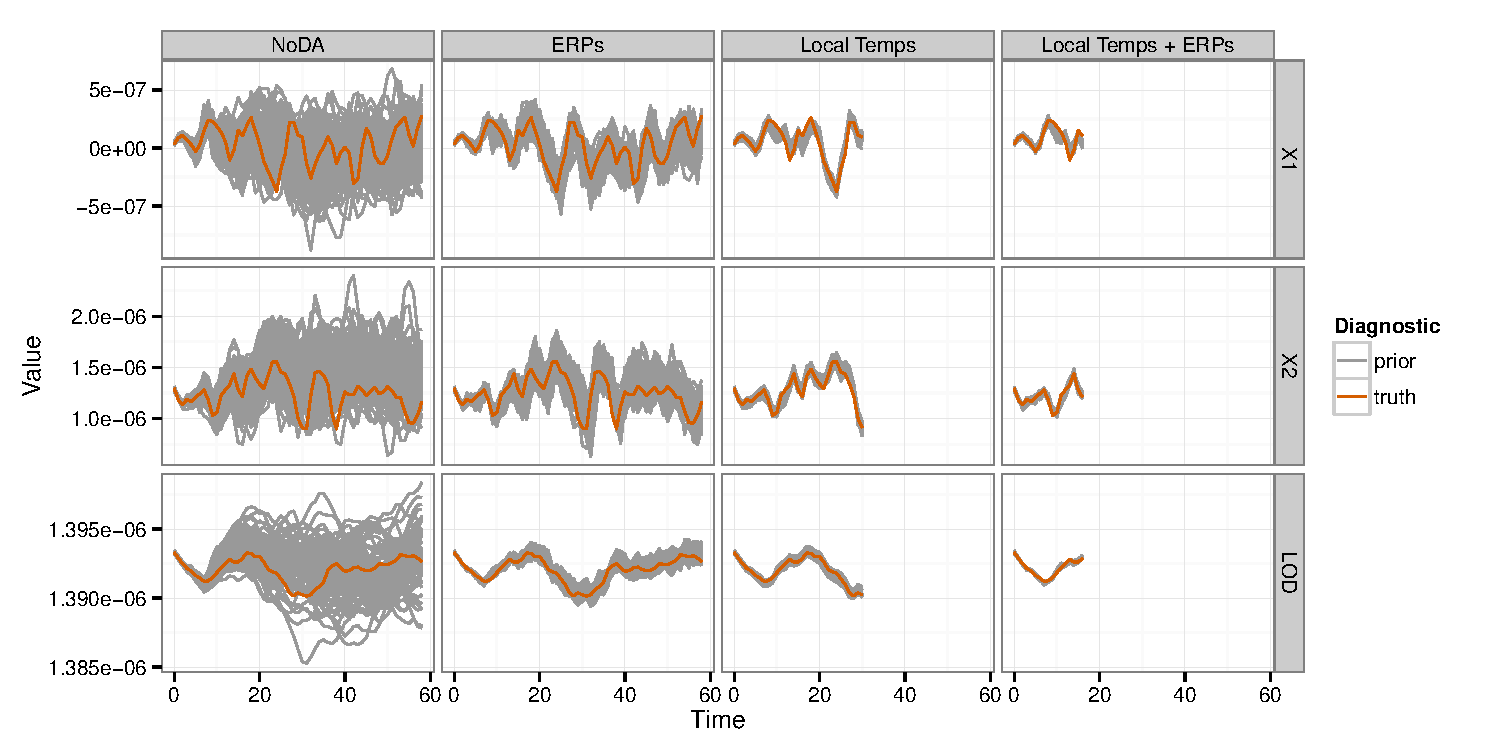
\includegraphics[width=\textwidth]{../../Documents/Plots/ERP_DA/paper/fit_to_ERPs.pdf} 
 \caption{ The DART prior ensemble (gray) compared to the true state (orange) in terms of assimilation time and each of the three angular momentum functions [(\ref{eq:X1})-(\ref{eq:X3}), (\ref{eq:X3_to_LOD})].  The columns compare the four experiments summarized in Table \ref{tab:expts}.  }
 \label{fig:fit_to_ERPs}
\end{figure}

%-----evolution of the covariances between local variables and the AAM observations
 \begin{figure}
	 \includegraphics[width=\textwidth]{Paper_figures/ERPDA_paper_U_to_LOD_covariances.pdf}
	 \caption{Evolution of the covariance between zonal wind and the axial angular momentum component ($\chi_3$), at 5-day intervals, assimilating observations of the three angular momentum components.}
 \label{fig:covariances}
\end{figure}

%-----evolution of the prior error and corresponding increments 
 \begin{figure}
	 \includegraphics[width=\textwidth]{Paper_figures/ERPDA_paper_U_priorerror_vs_increment.pdf}
	 \caption{Top row: evolution of the prior error (Truth-Prior) in the zonal wind, at 5-day intervals, assimilating observations of the three angular momentum components. Bottom row: the analysis increment (Posterior-Prior) in the zonal wind for the same times.} 
 \label{fig:error_increments}
\end{figure}

%-----error reduction in time  - stratosphere and tropopsphere  
 \begin{figure}
	 \includegraphics[width=\textwidth]{Paper_figures/ERPDA_paper_U_error_reduction.pdf}
	 \caption{Evolution of the difference in true error (Truth-Prior) when the three angular momentum components are assimilated, relative to no assimilation. Pink indicates a reduction in error relative to no assimilation. The first row shows error reduction in the troposphere (averaging between 100 and 500 hPa) and the second row shows error reduction in the stratosphere (averaging between 30hPa and the model top).}
	 \label{fig:ER}
\end{figure}

%-----focus on the ensemble in two regions to show how it is moved away from the true state
 \begin{figure}
	 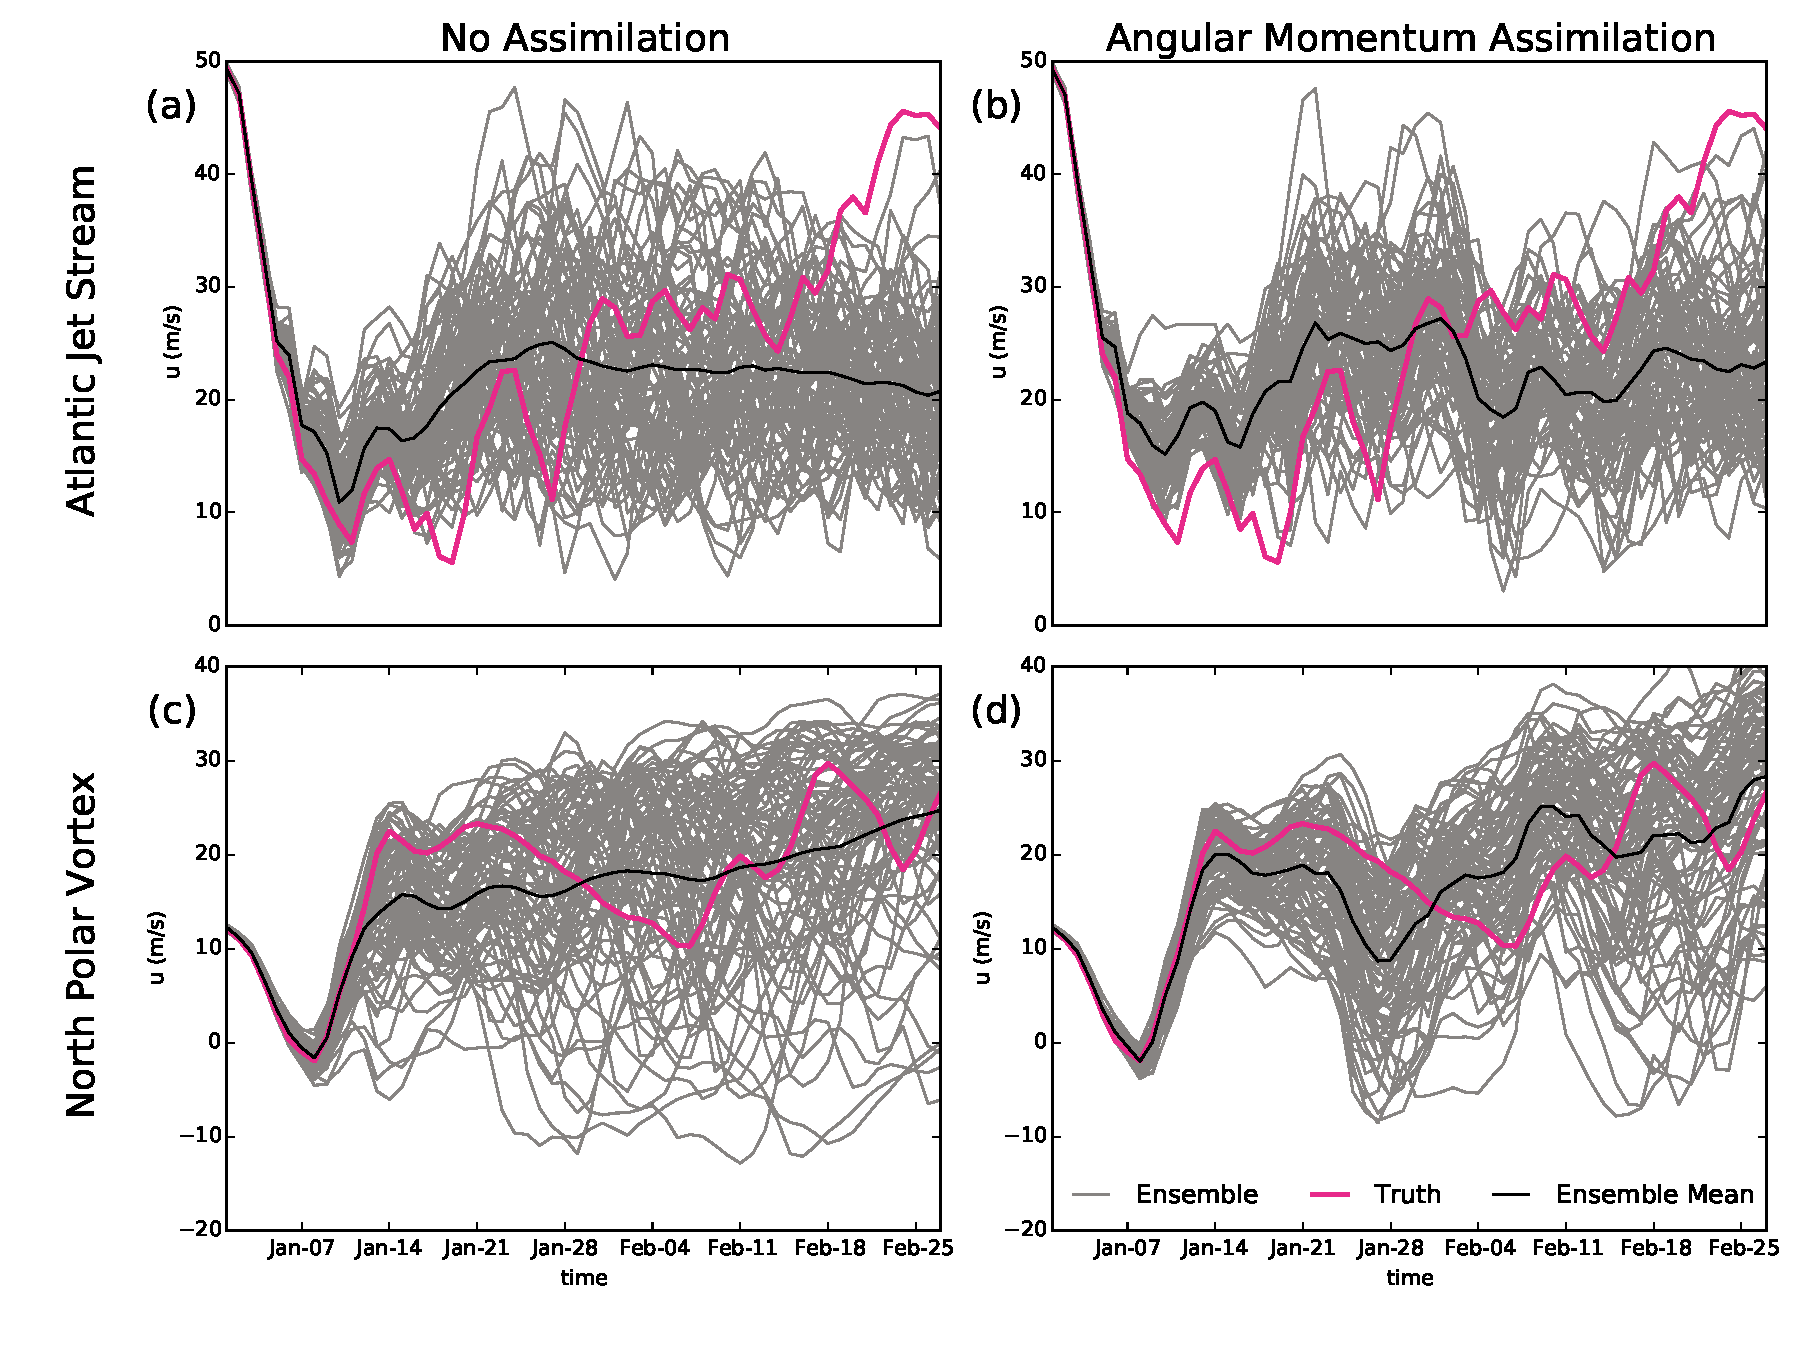
\includegraphics[width=\textwidth]{Paper_figures/ERPDA_paper_point_checks.pdf}
	 \caption{Comparison of the ensemble (gray) and its mean (black) to the true state (pink), for no assimilation (left column) and with assimilation of the three angular momentum components (right column). The top row shows zonal wind averaged over the North Atlantic jet (see text), and the bottom row shows zonal wind averaged in the polar vortex (see text).}
	 \label{fig:point_checks}
\end{figure}


%-----evolution of rank histograms to show filter divergence
% \begin{figure}
%	 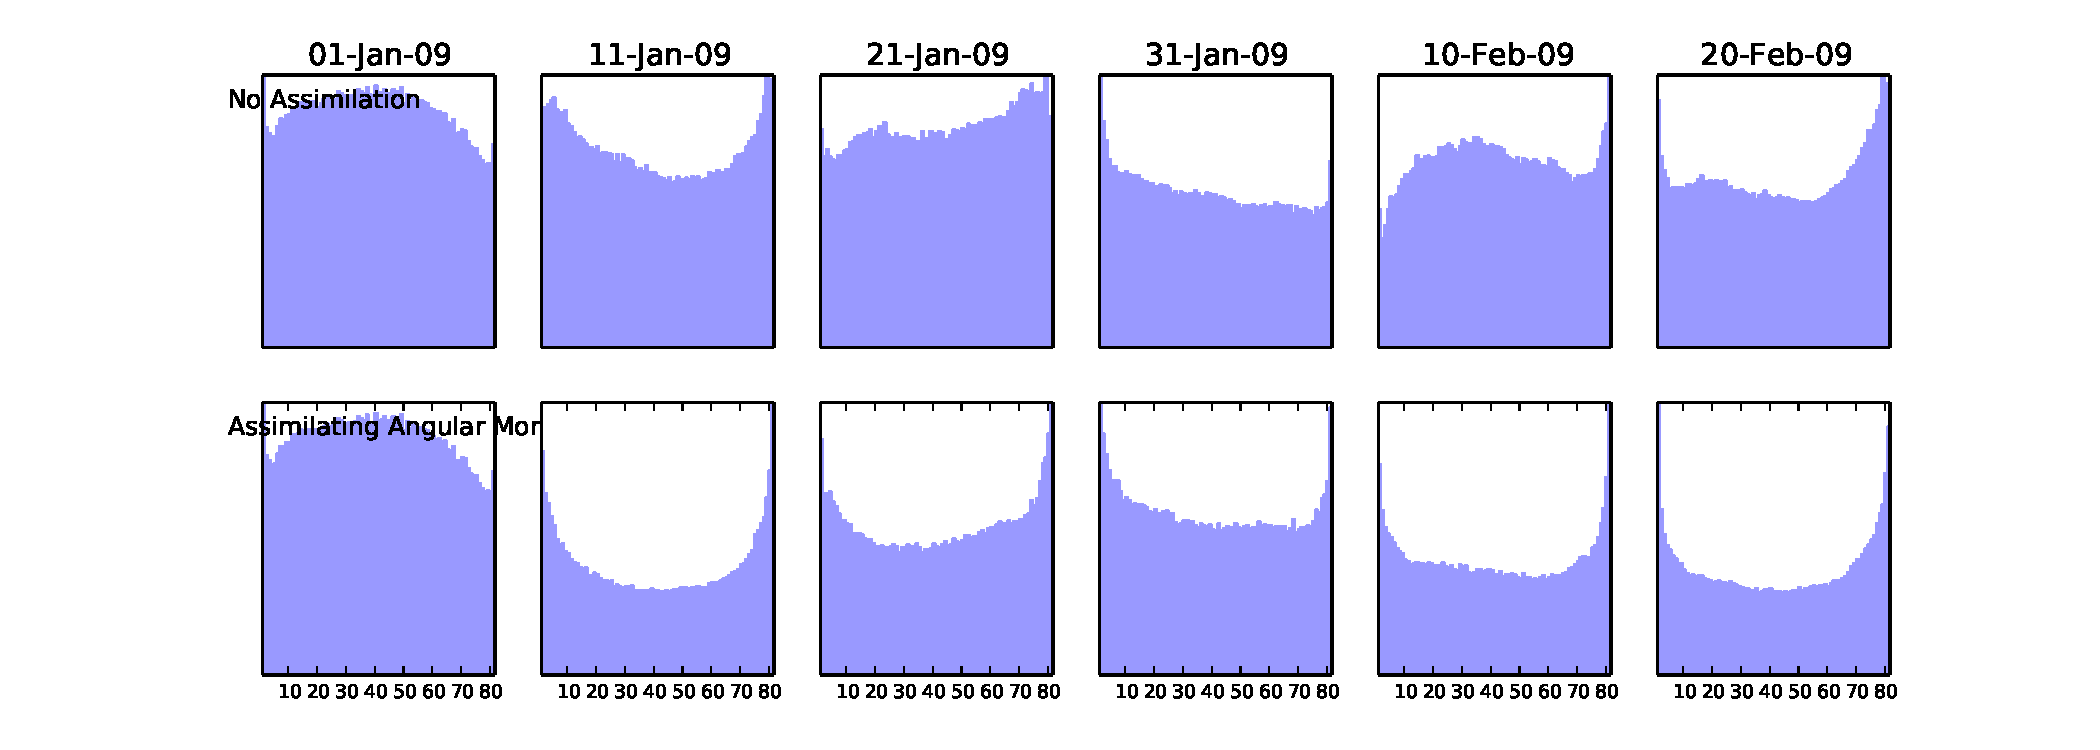
\includegraphics[width=\textwidth]{Paper_figures/ERPDA_paper_U_rank_histograms.pdf}
%	 \caption{Evolution of the rank histogram of the zonal wind field at 10-day intervals, for the run with no assimilation (top row) and assimilating the three components of angular momentum (bottom row).}
%	 \label{fig:RH}
%\end{figure}
